\newcommand{\DoNotLoadEpstopdf}{} % No EPS conversion or shell execution is needed.
\documentclass[11pt,letterpaper]{article}
\usepackage[T1]{fontenc}
\usepackage[utf8]{inputenc}
\usepackage[margin=.87in,top=.83in,bottom=.87in,headheight=23pt,headsep=.22in]{geometry}
\usepackage{amsmath,amsthm,mathtools}
\usepackage{newpxtext,newpxmath}
\usepackage{microtype}
\usepackage{booktabs,tabularx,array,longtable,multirow}
\usepackage{graphicx,xcolor,tikz,pgfplots}
\usetikzlibrary{arrows.meta,positioning,calc,fit,backgrounds,decorations.pathmorphing}
\pgfplotsset{compat=1.18}
\usepackage[most]{tcolorbox}
\usepackage{enumitem,needspace,fancyhdr,titlesec,caption,float,placeins}
\usepackage{listings,xurl,upquote}
\usepackage[numbers,sort&compress]{natbib}
\usepackage[unicode,bookmarksnumbered]{hyperref}
\usepackage{bookmark}
\definecolor{Ink}{HTML}{221A2D}
\definecolor{Violet}{HTML}{3E244B}
\definecolor{Gold}{HTML}{A87724}
\definecolor{LightGold}{HTML}{E4BF73}
\definecolor{Ivory}{HTML}{FBF8F0}
\definecolor{Muted}{HTML}{635C69}
\definecolor{Rule}{HTML}{D9CFBE}
\definecolor{Pale}{HTML}{F4F0F6}
\hypersetup{pdftitle={ALPHA GENESIS FLYWHEEL OMEGA: Three Orders of Intelligence},pdfauthor={Vincent Boucher},pdfsubject={Transformational Intelligence: frontier-coupled autonomous discovery, commercial compounding, and productive expansion},pdfkeywords={ALPHA GENESIS, SUCCESSOR OMEGA, transformational intelligence, autonomous discovery, frontier replay, scientific instruments, economic invention},colorlinks=true,linkcolor=Violet,citecolor=Violet,urlcolor=Violet}
\pagestyle{fancy}\fancyhf{}
\fancyhead[L]{\footnotesize\sffamily\color{Muted}ALPHA GENESIS FLYWHEEL $\Omega$}
\fancyhead[R]{\footnotesize\sffamily\color{Muted}Boucher \;|\; Research edition 2.0}
\fancyfoot[L]{\scriptsize\sffamily\color{Muted}TRANSFORMATIONAL INTELLIGENCE $\infty$}
\fancyfoot[R]{\small\color{Gold}\thepage}
\renewcommand{\headrulewidth}{.35pt}
\renewcommand{\headrule}{\hbox to\headwidth{\color{Rule}\leaders\hrule height \headrulewidth\hfill}}
\setlength{\parindent}{0pt}
\setlength{\parskip}{.48em plus .08em minus .05em}
\setlength{\emergencystretch}{2.5em}
\linespread{1.045}
\raggedbottom
\widowpenalty=10000
\clubpenalty=10000
\titleformat{\section}{\Large\bfseries\color{Violet}}{\color{Gold}\thesection}{.7em}{}
\titleformat{\subsection}{\large\bfseries\color{Ink}}{\thesubsection}{.7em}{}
\titleformat{\subsubsection}{\normalsize\bfseries\color{Ink}}{\thesubsubsection}{.7em}{}
\titlespacing*{\section}{0pt}{2.1ex plus .6ex minus .2ex}{.8ex}
\titlespacing*{\subsection}{0pt}{1.5ex plus .4ex minus .2ex}{.4ex}
\captionsetup{font=small,labelfont={bf,color=Violet},textfont={color=Muted},skip=7pt}
\setlist{leftmargin=1.4em,itemsep=.15em,topsep=.2em,parsep=0pt}
\renewcommand{\arraystretch}{1.16}
\newcolumntype{Y}{>{\raggedright\arraybackslash}X}
\newcolumntype{P}[1]{>{\raggedright\arraybackslash}p{#1}}
\newcommand{\E}{\mathbb{E}}
\newcommand{\Prob}{\mathbb{P}}
\newcommand{\I}{\mathcal{I}}
\newcommand{\R}{\mathcal{R}}
\newcommand{\Hh}{\mathcal{H}}
\newcommand{\GG}{\mathcal{G}}
\newcommand{\ind}{\mathbf{1}}
\newcommand{\OmegaName}{SUCCESSOR $\Omega$}
\newcommand{\Genesis}{GENESIS}
\DeclareMathOperator*{\argmax}{arg\,max}
\DeclareMathOperator*{\argmin}{arg\,min}
\DeclareMathOperator{\rank}{rank}
\newtheorem{definition}{Definition}[section]
\newtheorem{proposition}{Proposition}[section]
\theoremstyle{remark}\newtheorem{remark}{Remark}[section]
\newtcolorbox{thesisbox}{enhanced,breakable,colback=Ivory,colframe=Gold,boxrule=.5pt,arc=1.5mm,left=12pt,right=12pt,top=9pt,bottom=9pt,before skip=10pt,after skip=10pt}
\newtcolorbox{statusbox}{enhanced,breakable,colback=Pale,colframe=Violet,boxrule=0pt,borderline west={2.5pt}{0pt}{Violet},arc=0mm,left=11pt,right=11pt,top=8pt,bottom=8pt,before skip=9pt,after skip=9pt}
\newcommand{\smallhead}[1]{\par\smallskip{\sffamily\bfseries\color{Gold}#1}\par\smallskip}
\lstset{upquote=true,basicstyle=\small\ttfamily,breaklines=true,columns=fullflexible,keepspaces=true,showstringspaces=false,frame=single,rulecolor=\color{Rule},backgroundcolor=\color{Ivory},xleftmargin=5pt,xrightmargin=5pt,framesep=7pt}
\setcounter{tocdepth}{1}
\renewcommand{\topfraction}{.85}
\renewcommand{\textfraction}{.08}
\renewcommand{\floatpagefraction}{.8}

\newcommand{\HH}{\mathcal{H}}
\newcommand{\CalA}{\mathcal{A}}
\newcommand{\CC}{\mathcal{C}}
\newcommand{\VV}{\mathcal{V}}
\newcommand{\net}{\operatorname{net}}
\newcommand{\N}{\mathbb{N}}
\newcommand{\sourcefile}[1]{\texttt{\path{#1}}}
\newenvironment{keyidea}{\begin{thesisbox}\bfseries}{\end{thesisbox}}
\begin{document}

\begin{titlepage}
\thispagestyle{empty}

\begin{tikzpicture}[remember picture,overlay]
\fill[Ink] (current page.south west) rectangle (current page.north east);
\fill[Violet,opacity=.6] ([yshift=2.4in]current page.south west) rectangle ([yshift=-3.45in]current page.north east);
\draw[LightGold,line width=.8pt] ([xshift=.35in,yshift=.35in]current page.south west) rectangle ([xshift=-.35in,yshift=-.35in]current page.north east);
\draw[LightGold,opacity=.28,line width=.35pt] ([xshift=.43in,yshift=.43in]current page.south west) rectangle ([xshift=-.43in,yshift=-.43in]current page.north east);
\node[anchor=north west,text=LightGold,font=\sffamily\small] at ([xshift=.75in,yshift=-.7in]current page.north west) {MONTREAL.AI\quad /\quad QUEBEC.AI};
\node[anchor=north east,text=LightGold,font=\sffamily\small] at ([xshift=-.75in,yshift=-.7in]current page.north east) {RESEARCH EDITION 2.0};
\node[anchor=north,text=Ivory,font=\fontsize{28}{33}\selectfont] at ([yshift=-1.30in]current page.north) {ALPHA};
\node[anchor=north,text=LightGold,font=\fontsize{64}{70}\selectfont\bfseries] at ([yshift=-1.88in]current page.north) {GENESIS};
\node[anchor=north,text=Ivory,font=\fontsize{28}{33}\selectfont] at ([yshift=-2.90in]current page.north) {FLYWHEEL $\Omega$};
\node[anchor=north,align=center,text=Ivory,text width=6.6in,font=\fontsize{16}{21}\selectfont] at ([yshift=-3.58in]current page.north) {Turn the next advance in AI into your next ability\\to autonomously discover at scale.};
\coordinate (O) at ([yshift=-6.15in]current page.north);
\foreach \r in {1.00,1.10,1.43,1.51}{\draw[LightGold,opacity=.6,line width=.6pt] (O) circle (\r in);}
\foreach \ang in {0,60,120}{\draw[LightGold,opacity=.35,rotate around={\ang:(O)}] (O) ellipse (2.12in and .60in);}
\foreach \ang in {30,150,270}{\fill[LightGold] ($(O)+(\ang:1.43in)$) circle (4pt);\draw[LightGold,opacity=.5] ($(O)+(\ang:1.43in)$) circle (9pt);}
\node[text=LightGold,font=\fontsize{85}{90}\selectfont] at (O) {$\Omega$};
\node[text=Ivory,font=\sffamily\small,fill=Ink,inner sep=6pt] at ($(O)+(90:1.51in)$) {SEE THE FRONTIER};
\node[text=Ivory,font=\sffamily\small,fill=Ink,inner sep=6pt] at ($(O)+(210:1.83in)$) {SEE THE CONSEQUENCES};
\node[text=Ivory,font=\sffamily\small,fill=Ink,inner sep=6pt] at ($(O)+(330:1.83in)$) {IMPROVE THE INVENTOR};
\node[anchor=north,text=LightGold,font=\sffamily\bfseries\large] at ([yshift=-8.25in]current page.north) {RIDING THE EXPONENTIAL};
\node[anchor=north,text=Ivory,align=center,text width=6.4in,font=\large] at ([yshift=-8.68in]current page.north) {Build the advantage that discovers---\\and builds---the next advantage.};
\node[anchor=south west,text=Ivory,align=left,font=\normalsize] at ([xshift=.75in,yshift=.83in]current page.south west) {\textbf{Vincent Boucher}\\Montr\'{e}al, Qu\'{e}bec, Canada};
\node[anchor=south east,text=LightGold,align=right,font=\small] at ([xshift=-.75in,yshift=.83in]current page.south east) {TRANSFORMATIONAL INTELLIGENCE $\infty$\\4 November 2026};
\end{tikzpicture}
\null
\end{titlepage}
\setcounter{page}{1}

\begin{center}
{\sffamily\small\color{Gold}THE ADVANTAGE WORTH BUILDING}\par\medskip
{\LARGE\bfseries\color{Violet}ALPHA GENESIS FLYWHEEL $\Omega$}\par\medskip
{\large Riding the Exponential: Three Orders of Intelligence\\for an Enterprise That Discovers What Becomes Possible}\par\bigskip
Vincent Boucher\quad $\cdot$\quad MONTREAL.AI / QUEBEC.AI\par
{\small Montr\'{e}al, Qu\'{e}bec, Canada\quad $\cdot$\quad 4 November 2026}
\end{center}
\smallhead{ABSTRACT}
An advance in artificial intelligence is not yet an advantage for an enterprise. The missing step is to discover which valuable activities it makes attainable, construct the appropriate means, and learn from their use. We propose ALPHA GENESIS FLYWHEEL $\Omega$, a frontier-adaptive discovery enterprise organized around three orders of intelligence: see the frontier, see its consequences, and improve the machinery that discovers those consequences. Building on Transformational Intelligence, the institution may change representations, information channels, production methods, coordination, and economic arrangements while preserving the authorized purpose. Its methods are origin-neutral: an existing frontier agent is adopted when it is the best complete route; costly inheritance is retired; construction is funded only when its prospective value justifies its full costs. A capability hypergraph represents jointly enabling means, while a belief-aware planner compares direct use, composition, invention, experimentation, delay, and non-entry. MuZero supplies an important planning analogy, not a ready-made model of unknown industries. We formalize discovery versus selection error, decision-relevant information value, and conditional conversion-lag advantage. A reproducible finite study selects a diagnostic experiment with value 34.41, versus 31.30 for the strongest no-probe planner, and chooses existing tools or non-entry in adverse cases. Separately, source-matched native simulation completes six accepted deliveries and records US\$143.20 modeled profit; conventional routing ties the proposed selector and is retained. Neither result establishes real demand, general discovery superiority, or open-ended self-improvement. We specify the empirical programme needed to establish those claims and connect qualified capability construction to an economically sustained expansion of scientific and productive capacity.

\begin{statusbox}
\textbf{Research status.} A research synthesis, formal decision contracts, exact authored computations, and reproduced implementation checks. This edition is not a deployed discovery enterprise, a claim of new physical measurements, or evidence of actual customer revenue. \textbf{What is newly verified here:} an independent planning oracle, 54 parameter checks, four source-matched operating reproductions, and the completed 62-test native suite. The operational source remains the stated historical reference, not current-main qualification.
\end{statusbox}
{\small\textbf{Keywords:} transformational intelligence; frontier awareness; opportunity discovery; model-based planning; economic invention; capability inheritance; self-sustaining enterprise.}

\clearpage
\smallhead{THE PAPER AT A GLANCE}
\begin{keyidea}
New intelligence is an input.\\
A qualified capability is an asset.\\
A better way to discover valuable capabilities is the deeper advantage.
\end{keyidea}
\textbf{The question.} What valuable activity has just become technically or economically attainable, and what must be constructed to make it useful?

\textbf{The product hypothesis.} A customer-owned discovery application that accepts a consequential objective, authorized evidence and resources; constructs competing complete routes; produces usable artifacts; and explains what the evidence supports. The customer buys an ability, not a conversation among agents.

\textbf{The enterprise rule.} Use the best complete means, regardless of origin. Do not preserve internal machinery for prestige, reject an ordinary winner because it is ordinary, or book imagined successor benefits as present earnings.

\textbf{The compounding hypothesis.} A qualified invention can become an instrument, representation, or construction procedure that improves different successor work. That enabling relationship must be tested, not inferred from chronology or a growing archive.

\begin{figure}[H]
\centering
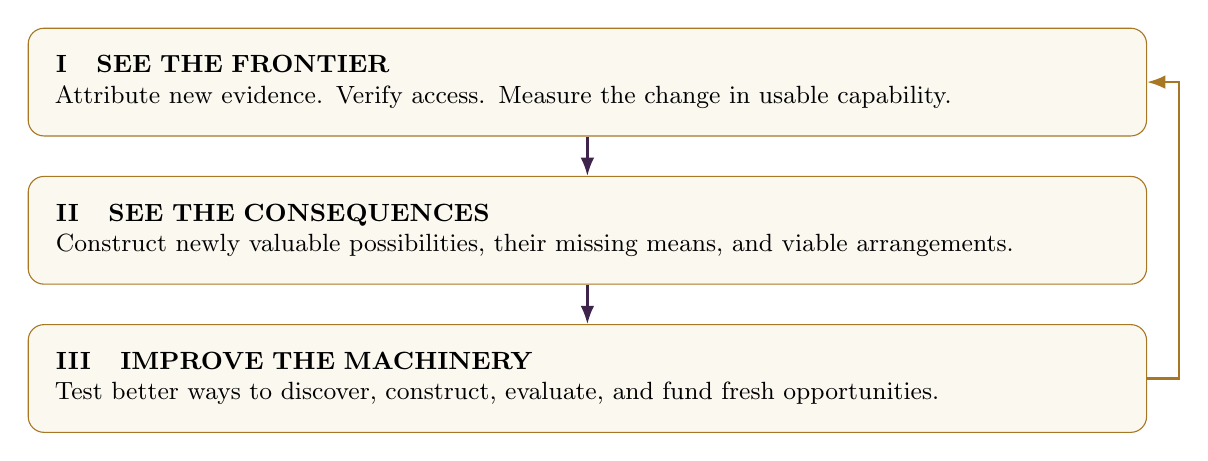
\begin{tikzpicture}[node distance=5mm,>=Latex,every node/.style={font=\small},
 stage/.style={draw=Gold,rounded corners=2mm,fill=Ivory,text width=13.5cm,align=left,inner sep=10pt}]
\node[stage] (one) {\textbf{I\quad SEE THE FRONTIER}\\Attribute new evidence. Verify access. Measure the change in usable capability.};
\node[stage,below=of one] (two) {\textbf{II\quad SEE THE CONSEQUENCES}\\Construct newly valuable possibilities, their missing means, and viable arrangements.};
\node[stage,below=of two] (three) {\textbf{III\quad IMPROVE THE MACHINERY}\\Test better ways to discover, construct, evaluate, and fund fresh opportunities.};
\draw[->,thick,Violet] (one) -- (two);
\draw[->,thick,Violet] (two) -- (three);
\draw[->,thick,Gold] (three.east) -- ++(.4,0) |- (one.east);
\end{tikzpicture}
\caption{Three operational functions, not a universal intelligence scale. Independent evidence connects them; successful operation at one order does not certify the next.}
\end{figure}
\textbf{Read by purpose.} Sections~\ref{sec:thesis}--\ref{sec:orders} explain the thesis and frontier. Sections~\ref{sec:world}--\ref{sec:economics} define the decision architecture. Sections~\ref{sec:experiments}--\ref{sec:native} report the computations and implementation. Sections~\ref{sec:product}--\ref{sec:horizon} develop the product, qualification programme, and physical horizon. Appendices provide derivations, reproduction, and the claim register.

\clearpage
\tableofcontents
\clearpage

\section{The advantage worth building}\label{sec:thesis}
The strategic opportunity is not merely to own a powerful answer generator. It is to build an institution that repeatedly turns improving intelligence into valuable new abilities. A model may become better at engineering; a measurement instrument may consequently become affordable; that instrument may enable a production process; and accepted production may supply resources for further construction. The valuable object is the supported relationship between these achievements, not an impressive list of them.

ALPHA GENESIS FLYWHEEL $\Omega$ is proposed as that institution. Its mandate is to become exceptionally effective at seeing what has just become possible, building what is most valuable, and improving its ability to discover the next opportunity. It joins an autonomous commercial flywheel to an inventive one, without making either's success depend on a false claim about the other. A fixed-capability operation can earn and reinvest surplus. An experimental method can improve research without yet finding a customer. The complete enterprise seeks a defensible connection between useful construction, accepted value, available resources, and fresh successor benefit \citep{boucher2026notes,boucher2026genesis}.

\subsection{Four achievements, not one score}
We distinguish \emph{commercial value}, \emph{scientific novelty}, \emph{incremental institutional contribution}, and \emph{improved invention}. An established algorithm can underpin a valuable business. A novel algorithm can have no economical application. A carefully designed workflow may improve delivery without improving how new workflows are discovered. A newer foundation model may improve every result while the surrounding institution adds no advantage.

These distinctions resolve a false opposition between using the frontier and competing with it. If an accessible frontier agent provides the best complete route, GENESIS should use it. That is an operating success, although it is not evidence that a proprietary constructor is superior. The additional institution must justify its opportunity selection, integration, acceptance, distribution, or renewal contribution after the overhead it introduces. It need not defeat every component it incorporates.

For an authorized mission $\I$, let $J_\I(s)$ denote an explicitly defined net outcome for complete system $s$. With a nonempty, disclosed comparison set $\mathcal B$,
\begin{equation}
\alpha_\I(s;\mathcal B)=J_\I(s)-\max_{b\in\mathcal B}J_\I(b).
\label{eq:alpha}
\end{equation}
The alternatives may include ordinary software, a direct frontier agent, a specialist, procurement, customer self-service, and non-entry. Hard requirements remain constraints. Where outcomes cannot legitimately be reduced to money or a scalar score, report the actual trade-offs instead of inventing an exchange rate. Equation~\eqref{eq:alpha} defines a comparison, not an estimate of all alternatives that might exist.

\subsection{Transform the means, not the success criterion}
The foundation is \emph{Transformational Intelligence: Learning to Change the Game} \citep{boucher2026ti}. Its separation of authorized purpose, problem formulation, and evaluation instrument is essential. A method's requirement is not necessarily the objective's requirement. If reliable delivery conventionally requires an expensive measurement, the enterprise can investigate a cheaper instrument, a selective measurement policy, or a production process that removes the uncertainty. It must preserve the outcome that made the work worth doing.

The representation, workflow, information channel, and interaction rules are therefore objects of invention. So are the procedures that invent them. But an agent cannot make a failed construction successful by lowering acceptance standards, treating a forecast as collected money, or changing the customer's purpose. Freedom over means is productive only when the outcome and authority remain accountable.

\begin{thesisbox}
\textbf{The founding hypothesis.} An origin-neutral institution that converts accessible frontier progress into qualified capabilities, economically useful delivery, and tested successor advantages can accumulate productive power beyond access to any single model.
\end{thesisbox}

\section{At the frontier: what changed, and what did not}\label{sec:frontier}
The evidence cutoff is \textbf{4 November 2026}. Table~\ref{tab:frontier} records selected developments relevant to the construction problem, not a claim of exhaustive awareness. Publication, demonstrated capability, account-level availability, and authorization to deploy are different facts. An announcement also does not establish that a task was impossible a week earlier.

\begin{table}[H]
\caption{A decision-relevant frontier snapshot. Provider announcements support their reported demonstrations, not the integrated performance of GENESIS.}\label{tab:frontier}
\small
\begin{tabularx}{\linewidth}{P{2.2cm}YY}
\toprule
\textbf{Date / source}&\textbf{What the source establishes}&\textbf{Consequence for this programme}\\
\midrule
3 Nov 2026\newline OpenAI & A device workflow connected mechanical design, electronics, and software; manufacturing still required review and iteration \citep{openai2026engineering}. & Construct connected engineering artifacts. Treat manufacturing qualification as work, not as a model prediction.\\
3 Nov 2026\newline DeepMind & Agentic cheminformatics connects scientific reasoning with executable domain tools and candidate generation \citep{google2026chem}. & Make a research skill executable. Computed candidates still need the applicable experimental evidence.\\
3 Nov update\newline Google Research & Computational Discovery adds an MCP integration route; the programme is described through a trusted tester channel \citep{google2026era}. & An agent can access strong existing discovery machinery where eligible. Do not assume access from a public description.\\
1 Nov revision\newline Hyperagents & The revised research describes editable task and meta-agent programs and reports improvements in evaluated domains \citep{hyperagents2026}. & Treat the improvement procedure as a candidate for improvement; compare against capable precedents.\\
9 Jul 2026\newline Google Cloud & AlphaEvolve is announced as generally available to Cloud customers on its agent platform \citep{google2026evolveaccess}. & It is a potential complete alternative, not merely an inaccessible research curiosity. Entitlement, costs, and authorization still matter.\\
Inspected\newline 4 Nov 2026 & OpenAI's mathematics repository contains manuscripts and proof artifacts at different verification stages, generated by an internal model \citep{openaimath2026}. & Investigate useful results and proof dependencies. Public artifacts do not provide access to their generating model.\\
\bottomrule
\end{tabularx}
\end{table}

OpenAI's engineering example is relevant because its residual manufacturing corrections identify a concrete integration gap. The chemistry workflow is relevant because language reasoning is coupled to explicit domain operations. The economic inference is ours: lowering the cost of connected construction may change which purpose-specific capabilities are worth producing. Neither source supplies a demand curve or proves that our proposed enterprise can capture that value.

The competitive bar is already high. AlphaEvolve combines generated code with automated evaluation \citep{alphaevolve2025}; ADAS searches executable agent designs \citep{adas2024}; and the Darwin G\"odel Machine investigates empirically evaluated self-modification \citep{dgm2025}. GENESIS should use applicable mechanisms from this work and compare with strong accessible alternatives. Generic orchestration, more agents, or a renamed search loop is insufficient differentiation.

\subsection{Riding the exponential is a conditional strategy}
The title names a strategy for adapting to rapid progress, not an empirical law that all useful capabilities grow exponentially. Some improve discontinuously, others stagnate, and deployment can remain limited by data, verification, access, or production. The enterprise should exploit improvements where observed and remain viable when a preferred frontier does not advance.

A simple conditional model makes the conversion issue precise. Suppose a relevant available capability index follows $F(t)=F_0e^{gt}$ over a stated interval, and institution $i$ converts it with effective lag $\tau_i$ and efficiency $\eta_i$:
\begin{equation}
Y_i(t)=\eta_iF(t-\tau_i),\qquad
\frac{Y_A(t)}{Y_B(t)}=\frac{\eta_A}{\eta_B}e^{g(\tau_B-\tau_A)}.
\label{eq:lag}
\end{equation}
This is an algebraic implication of the model. It is not a measured growth rate, a profit forecast, or a guarantee that faster adoption is better. Qualification effort can increase $\eta$ while increasing lag; premature deployment can destroy both. The optimization target is faster \emph{qualified conversion}, after failures and migration costs, not a race to install every release.

When all flows are expressed in the same units of accepted outcomes per unit time, useful throughput is additionally bounded by the smallest of construction, verification, delivery, and demand capacity. Improving only the model does not remove those other bottlenecks. The valuable frontier may be an instrument that changes one of them.

\section{Three orders of intelligence}\label{sec:orders}
The three orders describe operating functions and corresponding evidence requirements. They are neither an established scale of general intelligence nor a claim that an application acquires superintelligence by naming its stages.

\subsection{First order: see the frontier}
The observatory asks: \emph{What changed that could alter a decision?} It combines broad model knowledge with current primary sources, executable capability probes, access records, and failures observed in use. A frontier LLM is a powerful proposal and interpretation resource, but its internal knowledge is not a source of live access status, current price, or a verified scientific conclusion.

A useful frontier record binds the source and version to its publication time, observation time, claimed change, observed task behavior, prerequisites, access status, cost evidence, and expiry or invalidation conditions. Corrections, retractions, revoked permissions, and regressions are events too. A public statement that a model can design a circuit should not be converted directly into permission to fabricate or a claim that a particular board is safe.

Awareness is measured over declared source and task populations. Relevant-release recall, detection delay, source correctness, and the cost of verification are useful. ``Everything relevant'' has no observable universal denominator. Independent horizon scans and deliberately different retrieval methods can expose omissions in the institution's own catalogue. They cannot prove omniscience.

The observatory should prioritize evidence by the decision it may change. Reading another hundred articles about a capability already well understood may be inferior to checking one unresolved access or reliability condition. Conversely, attention focused exclusively on today's backlog can miss a new class of activity. Targeted monitoring and deliberate exploration must therefore coexist.

\subsection{Second order: see the consequences}
The consequence engine asks: \emph{What becomes worth doing because this change occurred?} It searches beyond applications that merely substitute cheaper inference into an unchanged product. A capability might enable a new observation, make a costly experiment economical, remove an engineering dependency, or create an acceptance procedure that allows a different commercial arrangement.

Its object is the \emph{complete productive arrangement}: beneficiary, useful outcome, productive means, evidence, participant incentives, resource commitments, and viable timing. A product that is technically feasible but cannot be verified, afforded, distributed, or voluntarily purchased is not a completed opportunity. These are construction targets, not reasons to assume the market will eventually cooperate.

Search proceeds in both directions. Backward reasoning identifies what blocks a valuable outcome. Forward reasoning asks what newly available means could enable. Their intersection proposes a construction. Cross-domain structural transfer can suggest relationships that topical retrieval misses; a verified failure can reveal the missing interface; and an alternative formulation can eliminate the need for that interface entirely \citep{boucher2026notes}.

The engine must retain rival hypotheses: the installed route may already suffice, the new capability may be irrelevant, or a simpler direct agent may win. Generation is not endorsement. Each proposal needs an executable path and a discriminating test before substantial commitment.

\subsection{Third order: improve the machinery that sees possibilities}
The third order asks: \emph{Which change would make future opportunity discovery and construction more effective?} The object can be a representation, search policy, experimental strategy, retrieval method, risk estimate, tool interface, or the procedure that proposes such changes.

A useful inheritance is more than a transcript. It may contain a working instrument, an applicability model, and a procedure for constructing related instruments. These are distinct assets. Only the first may initially have evidence. The deeper gain occurs when a retained procedure improves fresh construction, not merely when a new task reuses a prebuilt answer.

DreamCoder supplies a bounded precedent for learned abstractions supporting subsequent program search; POET supplies one for co-developing environments and solutions with transfer \citep{dreamcoder2020,poet2019}. Hyperagents directly makes the modification procedure editable in its evaluated systems \citep{hyperagents2026}. Our proposed enterprise extension concerns whether such mechanisms improve economically consequential discovery under complete resource accounting and changing external capability.

An updated foundation model, a richer initial archive, and a better discovery procedure can all improve results. The third-order claim must separate them. Without that separation, the institution can simply inherit progress made elsewhere and call it self-improvement.

\section{A living model of productive possibility}\label{sec:world}
We propose a hybrid model rather than a single neural network expected to know the economy. It contains an authoritative resource and permissions layer, a source-grounded capability representation, probabilistic beliefs about unresolved mechanisms and markets, and generators that propose new executable actions. The model is useful only insofar as it improves real decisions.

\subsection{Capabilities are conditional operations}
A capability record describes what an operation accepts, produces, consumes, and changes; where its evidence applies; which rights and dependencies it requires; and how it can fail. Access, qualification, and economic attractiveness are separate attributes. An operation can be accessible but unreliable, reliable but unsuitable, or useful but unaffordable under the present commitment schedule.

Let $\HH_t$ denote the qualified capability stock and $\GG_t$ a directed hypergraph of possible enabling relationships. A hyperedge $\{h_1,\ldots,h_k\}\rightarrow h'$ indicates that several prerequisites together may enable a construction. It must carry its assumptions, realization, cost, and evidence status. A hypothesis edge is not a qualified causal fact. Circular descriptions of mutual enablement do not supply a feasible bootstrap sequence.

This representation matters because a collection of individually weak components can be jointly enabling. An instrument without calibration may have little value; calibration without an instrument may have no use. Their bundle may make a useful distinction measurable. A greedy rule that admits only individually profitable additions can miss the combination. Section~\ref{sec:experiments} gives a transparent numerical example, not an algorithmic novelty claim.

\subsection{The graph must not become the boundary of imagination}
A finite capability graph is an instrument for reasoning, not an exhaustive map of reality. Frontier agents should be allowed to propose operations and representations outside its existing grammar. Such proposals enter a development environment with explicit effects and checking requirements; they do not grant themselves execution authority.

There are three different questions. Can an existing planner find a route through known operations? Can a constructor implement a proposed new operation? Can an open-world generator discover that operation or a valuable outcome not already supplied? The current prototypes primarily address the first and parts of the second. Solving an authored graph exactly does not settle the third.

A practical diagnosis records whether a failure comes from unavailable evidence, inadequate reasoning, insufficient resources, physical constraints, an avoidable dependency, or an inaccurate model of buyer behavior. Repeated failure alone is not proof of impossibility. Likewise, saying ``reframe the problem'' does not create a missing observation.

\begin{figure}[H]
\centering
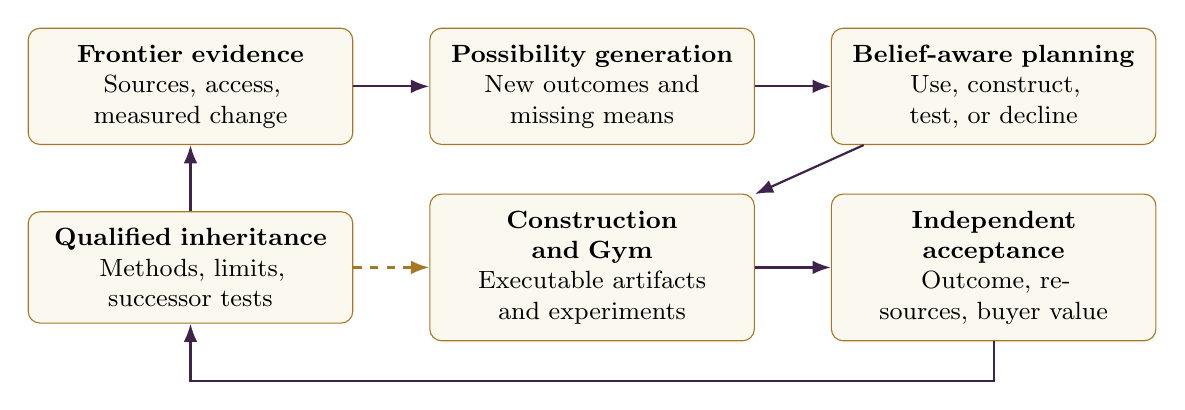
\begin{tikzpicture}[>=Latex,every node/.style={font=\small},
 box/.style={draw=Gold,fill=Ivory,rounded corners=1.5mm,align=center,text width=3.7cm,minimum height=1.2cm,inner sep=6pt}]
\node[box] (front) at (0,0) {\textbf{Frontier evidence}\\Sources, access, measured change};
\node[box] (gen) at (5.1,0) {\textbf{Possibility generation}\\New outcomes and missing means};
\node[box] (plan) at (10.2,0) {\textbf{Belief-aware planning}\\Use, construct, test, or decline};
\node[box] (ret) at (0,-2.3) {\textbf{Qualified inheritance}\\Methods, limits, successor tests};
\node[box] (gym) at (5.1,-2.3) {\textbf{Construction and Gym}\\Executable artifacts and experiments};
\node[box] (val) at (10.2,-2.3) {\textbf{Independent acceptance}\\Outcome, resources, buyer value};
\draw[->,thick,Violet] (front) -- (gen);
\draw[->,thick,Violet] (gen) -- (plan);
\draw[->,thick,Violet] (plan) -- (gym);
\draw[->,thick,Violet] (gym) -- (val);
\draw[->,thick,Violet] (val.south) -- ++(0,-.5) -| (ret.south);
\draw[->,thick,Violet] (ret) -- (front);
\draw[->,thick,Gold,dashed] (ret) -- (gym);
\end{tikzpicture}
\caption{Proposed information and construction loop. The independent acceptance boundary and authoritative resource controls constrain every path; they are not editable rewards owned by the candidate.}
\end{figure}

\section{MuZero is a planning inspiration, not the whole enterprise}\label{sec:muzero}
MuZero learns representations and latent transitions sufficient to predict decision-relevant reward, policy, and value, then plans with a learned model. Its reported evaluation covers Atari, Go, chess, and shogi \citep{muzero2020}. The important lesson is that a planner need not reconstruct every physical detail to make useful predictions. The inference that this already supplies an open-world scientific or commercial discovery engine would be unwarranted.

GENESIS faces different conditions: new tools can change the action repertoire; scientific experiments may be expensive and irreversible; market responses are strategic; observations are partial; access can disappear; and rewards may arrive late. A compelling imagined trajectory is not independent evidence of its physical or commercial feasibility.

\begin{table}[H]
\caption{Methods to incorporate when warranted, not a compulsory stack. The architecture should be allowed to simplify.}
\small
\begin{tabularx}{\linewidth}{P{3.0cm}YY}
\toprule
\textbf{Method}&\textbf{Useful contribution}&\textbf{What it does not establish here}\\
\midrule
Exact decision trees / dynamic programming & Transparent optimization in small declared models; independent reference calculations. & Optimal discovery outside the authored state and action space.\\
Bayes-adaptive planning \citep{bayesadaptive2007} & Joint reasoning about uncertain dynamics and actions that improve information. & Correct priors, an exhaustive hypothesis set, or calibrated market forecasts.\\
MuZero / sampled-action planning \citep{muzero2020,sampledmuzero2021} & Learned decision-relevant dynamics and search over promising actions. & Autonomous invention of arbitrary action semantics or a valid model of the economy.\\
Dreamer-style world models \citep{dreamer2025} & Learning policies using imagined trajectories in evaluated control settings. & That imagined scientific or commercial outcomes are externally valid.\\
Executable evolutionary construction \citep{alphaevolve2025,adas2024} & Generate and evaluate algorithms or agent designs. & Demand, financing, or general discovery advantage in our application.\\
Editable improvement procedures \citep{dgm2025,hyperagents2026} & Treat the machinery of improvement as an experimental object. & Unrestricted, indefinitely accelerating self-improvement.\\
\bottomrule
\end{tabularx}
\end{table}

The immediate engineering choice is a small, inspectable planner with explicit uncertainty, supplemented by strong proposal generators and conventional specialist tools. Learned planning becomes a challenger when the institution has enough relevant interaction evidence to train and calibrate it. The choice should be earned against exact or simpler approximate methods on the same decision requirements, including training, search, validation, and inference costs.

\subsection{Separate learned predictions from authoritative facts}
Model-predicted revenue is not a collection. An estimated probability of customer acceptance is not consent. A learned transition predicting access to a tool does not create access. The planner may reason probabilistically about each, but the execution layer must obtain the actual evidence or authorization required for the action.

The symbolic layer therefore preserves cash, obligations, identities, resource limits, and grants of authority. Learned components estimate consequences and propose constructions. This division is not a claim that symbolic records are infallible; their implementations need checking. It prevents a plausible forecast from silently becoming an operating permission.

\section{The decision contract: discover, select, and learn}\label{sec:decision}
Let $x_t=(b_t,\HH_t,\GG_t,c_t,o_t,\ell_t)$ contain beliefs, capabilities, enabling hypotheses, available cash, obligations, and remaining time or other finite resources. The authorized action set may include direct use, procurement, partnership, composition, construction, an experiment, delay, retirement, and stopping. Actions can alter future capabilities as well as beliefs.

For a finite horizon, one risk-neutral reference problem is
\begin{equation}
V_t(x)=\max_{a\in\CalA_{\mathrm{feasible}}(x)}
\E\!\left[r_t(x,a,Z)-k_t(x,a,Z)+\gamma V_{t+1}(x')\mid x,a\right].
\label{eq:bellman}
\end{equation}
Here $r_t$ and $k_t$ are incremental realized-value and cost quantities in declared common units, and $Z$ is the uncertain outcome. The transition tracks resource commitments and settlement timing. A terminal value, if used, must have a stated realizable interpretation. Future option value already represented in $V$ must not be added again as a separate bonus. Hard safety, permission, quality, and liquidity requirements belong in feasibility, not as penalties that high predicted profit can simply outweigh.

Equation~\eqref{eq:bellman} is a model-based decision specification, not a solved game for the actual enterprise. Risk preferences, robustness requirements, and incomplete models may demand other formulations. In every case, the forecast distribution, feasible set, solution method, and approximation gap should be stated. ``Game-theoretically optimal'' is not meaningful without players, information, strategies, timing, incentives, and a solved or bounded comparison.

\subsection{Discovery error is not selection error}
A perfect selector can choose only among the possibilities it receives. For an analytically specified universe of feasible arrangements with values $J(a)$, let $V^*=\sup_a J(a)$ and let $C$ be the nonempty candidate set produced by a discovery process. Then
\begin{equation}
V^*-J(\hat a)=
\underbrace{V^*-\max_{a\in C}J(a)}_{\text{discovery gap}}+
\underbrace{\max_{a\in C}J(a)-J(\hat a)}_{\text{selection gap}}.
\label{eq:gaps}
\end{equation}
This identity separates two targets; it does not estimate either in an open world. A finite planner may have zero selection gap in its model while overlooking the most valuable application. A larger candidate list can also be worse after the costs of generating, integrating, and checking it. Complete discovery campaigns, rather than final plans alone, must be compared.

\begin{proposition}[Conditional selection bound]
For a declared finite candidate set $C$, suppose $|\hat J(a)-J(a)|\leq\epsilon$ for every $a\in C$ and $\hat J(\hat a)\geq\max_{a\in C}\hat J(a)-\delta$. Then
\begin{equation}
\max_{a\in C}J(a)-J(\hat a)\leq 2\epsilon+\delta.
\label{eq:selection}
\end{equation}
\end{proposition}
\begin{proof}
For a maximizer $a^*$ in $C$, $J(a^*)\leq\hat J(a^*)+\epsilon\leq\hat J(\hat a)+\delta+\epsilon\leq J(\hat a)+\delta+2\epsilon$.
\end{proof}
This elementary bound clarifies the priority of calibrated values and adequate candidate generation. An exact optimizer does not compensate for confidently wrong economics. Uniform error control must be justified; assigning a small $\epsilon$ does not establish it. No term in the bound covers opportunities absent from $C$.

\subsection{Buy information when it changes the decision}
For an experiment $e$ with outcome $Z$, a one-step value-of-information comparison is
\begin{equation}
\operatorname{VOI}(e)=
\E_Z\!\left[\max_{a\in A(Z)}\E[J(a)\mid Z,e]\right]
-\max_{a\in A_0}\E[J(a)]-K_e.
\label{eq:voi}
\end{equation}
$K_e$ includes the applicable experiment, interpretation, delay, and opportunity costs. A sequential problem must include the consumed time and resources in the transition rather than subtract them twice. The post-experiment feasible set may change because the experiment constructs a useful instrument, but that effect requires an actual construction and a validated applicability claim.

A measurement can be highly informative yet economically irrelevant if no subsequent action changes. Conversely, a small amount of information can be valuable when it avoids an expensive mistaken build. Cases where no useful affordable experiment is found, where neither initial hypothesis is correct, and where stopping is best are part of the specification, not embarrassments to suppress.

\subsection{Retain the contribution, not the sunk cost}
The prospective value of retaining capability $h$ is the best achievable continuation with it, net of its future carrying and adaptation costs, compared with the best continuation without it. The latter may buy or construct an alternative. Historical acquisition cost remains in programme accounting, but is not charged a second time merely to decide whether an already acquired capability should stay active.

A cheap inert archive, an actively maintained executable tool, and a production-qualified service have different costs. Retiring one need not erase the evidence behind another. Complementary capabilities should be assessed jointly when their contribution depends on a bundle. Neither ``retain everything'' nor ``delete anything without standalone revenue'' is an adequate policy.

\section{Frontier Replay: turn a release into a changed opportunity}\label{sec:replay}
Frontier Replay is the proposed operational bridge between awareness and construction. The institution preserves a compact record of valuable unresolved opportunities: the intended outcome, strongest complete alternative, suspected obstruction, attempted means, incurred costs, and evidence that could change the next decision. It does not treat failed attempts as permanently impossible or as an obligation to continue indefinitely.

When a new capability becomes accessible, replay begins with a specific counterfactual: \emph{Would this change remove the obstacle that mattered?} A stronger numerical coder may reopen a failed solver construction. A better engineering interface may make a fixture manufacturable. A new experimental result may invalidate the original opportunity entirely. Each is a legitimate frontier consequence.

\subsection{A capability delta, not a release name}
The useful input is a measured or testable difference in capability, cost, reliability, or access. A large benchmark improvement can be irrelevant to a particular customer outcome. A small reduction in a previously dominant integration cost can change feasibility. The application should therefore bind a frontier event to the dependency it is alleged to change, not merely attach the newest model label to an old workflow.

A replay record should answer five compact questions: what changed; which opportunity might be affected; which enabling link is uncertain; what executable test distinguishes the alternatives; and what action follows each plausible outcome. The test can select the incumbent, retire a capability, or choose non-entry. A repeated comparison is not fresh confirmation when its outcomes have already influenced development.

\subsection{A productive replay episode}
The following is an operating specification, not a claim that the released prototypes execute every step:
\begin{enumerate}
\item Verify the event, access, scope, and applicable authority. Preserve uncertainty where evidence is missing.
\item Generate materially different consequences, including a direct existing-tool route and an option that avoids the assumed construction.
\item Compare complete prospective value and feasible funding sequences. Select an informative test or construction only when warranted.
\item Build and challenge in the development environment; record failed branches and resource consumption.
\item Freeze the candidate and assess it on fresh work under the original outcome requirements.
\item Deliver within its supported scope, reconcile actual obligations, and test any claimed successor contribution separately.
\end{enumerate}

Backlog replay must coexist with de-novo opportunity discovery. Otherwise, the institution only revisits questions it knew to ask before the frontier changed. Search budgets should be explicit, but no permanent field catalogue or fixed percentage of spending is inherently optimal. Allocation itself is a candidate for experimentally demonstrated improvement.

\section{The enterprise: value, participation, and feasible continuation}\label{sec:economics}
The customer promise is a useful capability that the buyer prefers to its complete alternatives. The enterprise should search the outcome, production method, verification process, commercial arrangement, and financing path together. Better production economics are insufficient when the buyer's alternative improves even faster.

\subsection{The price window describes a construction problem}
In a stated quasilinear model, let $v_i$ be buyer $i$'s expected value of an accepted outcome, $u_i^{\mathrm{out}}$ the utility of its best alternative, and $b_i$ its non-price burden. Voluntary participation requires
\begin{equation}
p_i\leq v_i-u_i^{\mathrm{out}}-b_i.
\label{eq:buyer}
\end{equation}
The burden includes the buyer's own setup, compute, attention, integration, risk, and residual checking. For $n$ accepted deliveries, fixed lifecycle cost $F$, per-delivery cost $c$, and required total surplus $m$, a common viable price additionally needs
\begin{equation}
p\geq c+\frac{F+m}{n}.
\label{eq:seller}
\end{equation}
These are feasibility inequalities under their assumptions, not a market-equilibrium solution. They identify what might need to change: improve value, lower complete costs, reduce the buyer's burden, or reach additional real demand. The variable $n$ cannot be enlarged on paper without buyers, capacity, acquisition, and funded obligations.

A technically excellent construction with no plausible price window should be declined or reformulated. An intermediate instrument can still be justified when its credible downstream contribution or decision value exceeds its complete cost. Its hypothetical future benefit is not earned revenue, collateral already secured, or unrestricted cash.

\subsection{Competition can help society while compressing our margin}
A public capability is available to rivals and customers as well as to GENESIS. They may develop cheaper alternatives, copy an application, or change the terms of participation. A rational enterprise must model these responses when material, including the buyer's option to do the work itself or decline.

An authored arithmetic counterexample makes the point. If a buyer's maximum acceptable price is 130 and our complete unit cost is 100, the price-ceiling margin is 30. A public advance might reduce cost to 40 while lowering the acceptable price to 60 because outside options improve. The margin becomes 20, despite a much better production capability. These are illustrative numbers, not observed willingness to pay.

Potential defensibility comes from demonstrated conversion ability, qualified interfaces, distribution, appropriately permissioned knowledge, useful experimental assets, and reliable delivery. None supplies an automatic monopoly. The operating question is whether that integrated contribution remains worth its cost as alternatives improve.

\subsection{A self-sustaining enterprise is a cash-and-obligations claim}
Let $C_t$ be cash, $P_t$ protected obligations and reserves, and $A_t=C_t-P_t$ available cash under a declared accounting convention. A construction is currently financeable only if its required commitments are supported by actual available resources and permissible financing. Positive expected terminal profit does not by itself satisfy that condition.

The accounting path is:
\begin{center}
\small
Offer $\rightarrow$ voluntary purchase $\rightarrow$ funding $\rightarrow$ production $\rightarrow$ acceptance\\
$\rightarrow$ collection $\rightarrow$ obligations covered $\rightarrow$ justified continuation.
\end{center}
An invoice is not a collection. Customer advances remain obligations until earned. Investment proceeds are not operating revenue. Modelled receipts are not actual funds. No parallel planning ledger should replace the native account that authorizes commitments.

For a stated horizon, an operational self-sustainability claim needs repeated accepted delivery, complete economic costs, sufficient liquidity through the path, and a supported continuation policy without unreported capital injections. This does not forbid legitimate financing. It requires financing to be distinguished from earned-funded growth and its terms to be accounted for. Seed-funded protection reserves can remain essential even when current operating expenditures are paid from earnings.

\subsection{Two flywheels, several sources of progress}
The \emph{commercial flywheel} repeats worthwhile delivery and uses available surplus for productive continuation. The \emph{invention flywheel} constructs qualified means and tests their contribution to new work. A third-order gain improves the procedure for finding those means. Exogenous foundation-model progress is a fourth source of improvement, not a substitute for evidence of the other three.

There is no requirement that the enterprise invent on every cycle. When direct delivery or distribution is the best investment, it should win. Conversely, an instrument that creates substantial future opportunity can be worth constructing before it earns standalone revenue. What matters is justified prospective value, feasible resources, and evidence of the enabling relationship, not adherence to a permanent research-spending ritual.

\section{Exact decision studies: what the planner actually chooses}\label{sec:experiments}
This edition re-executes the supplied finite Bayesian planner \citep{decision001} and adds a separately implemented oracle. The oracle re-creates the transitions in its own tuple-state recursion; it does not call the producer's action or outcome functions. Exact rational arithmetic avoids sampling uncertainty within this authored model. There is no trained MuZero network, model API call, live market, or discovered action grammar in this study.

\subsection{A disclosed finite world}
There are two hypothetical markets, $A$ and $B$, each deliverable once, and four decision steps. Starting cash is 25 model units and the protected reserve is 10. An existing frontier route has net returns 14 and 16; a specialist has 10 and 12. Constructing a candidate instrument costs 12. With prior probability $7/20$, it succeeds and supports returns 32 and 36, with zero per-delivery carrying cost in the base case. Otherwise, it adds no useful delivery ability. Construction reveals viability perfectly in this finite world; this strong assumption is not an empirical property of research.

Before construction, the planner may buy one diagnostic signal for 3 units. Its sensitivity is $9/10$ and false-positive probability $1/10$. Both experiment and construction consume a decision step. Acquisition must leave the protected reserve intact. Non-entry is always available. The return parameters and likelihoods are stipulated, not learned from buyers or current model releases.

The state tracks horizon, cash, posterior belief, whether the experiment or construction has occurred, and which markets have been served. The reference computes the strongest continuation over all permitted actions, including using an existing tool first to change later liquidity. This avoids comparing the candidate only with a weak, purely myopic policy.

\begin{table}[H]
\caption{Exact authored decision results. Values are model units, not observed dollars. The independent recursion agrees in each case.}\label{tab:decision}
\small
\begin{tabularx}{\linewidth}{Y P{2.7cm} r r r}
\toprule
\textbf{Case}&\textbf{Selected first action}&\textbf{Full plan}&\textbf{No probe}&\textbf{Direct only}\\
\midrule
Uncertain useful instrument & Buy diagnostic & 34.41 & 31.30 & 30.00\\
Existing frontier returns rise to 28 and 30 & Use frontier route & 58.00 & 58.00 & 58.00\\
Carrying cost rises to 25 per use & Use frontier route & 30.00 & 30.00 & 30.00\\
Every delivery route has negative net return & Stop & 0.00 & 0.00 & 0.00\\
\bottomrule
\end{tabularx}
\end{table}

The baseline diagnostic is positive with probability $19/50$, producing posterior $63/76$; the best next action is construction. A negative result has probability $31/50$ and posterior $7/124$; the best continuation uses existing frontier delivery. The full value is $3441/100=34.41$. The strongest planner forbidden to probe obtains $313/10=31.30$, so the net value of access to the diagnostic is $311/100=3.11$.

The often tempting comparison with direct delivery alone gives $34.41-30=4.41$. That is a weaker comparison. The paper uses the stronger 3.11 difference for the information claim. Perfect initial information, before charging for its acquisition, has value 39.10; the corresponding improvement over the strongest no-probe plan is 7.80. These values apply only to the stated horizon, resource rules, likelihoods, and payoffs.

\begin{figure}[H]
\centering
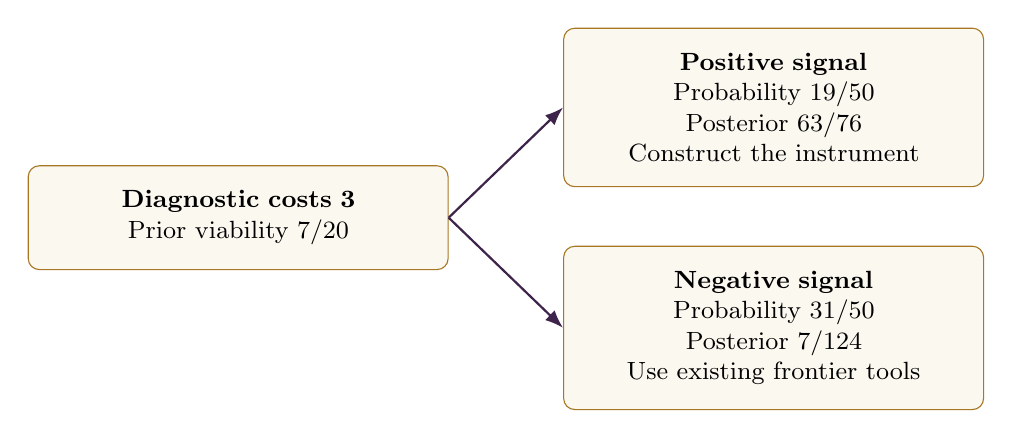
\begin{tikzpicture}[>=Latex,every node/.style={font=\small},
 box/.style={draw=Gold,fill=Ivory,rounded corners,align=center,text width=4.7cm,inner sep=9pt}]
\node[box] (probe) at (0,0) {\textbf{Diagnostic costs 3}\\Prior viability $7/20$};
\node[box] (yes) at (6.8,1.4) {\textbf{Positive signal}\\Probability $19/50$\\Posterior $63/76$\\Construct the instrument};
\node[box] (no) at (6.8,-1.4) {\textbf{Negative signal}\\Probability $31/50$\\Posterior $7/124$\\Use existing frontier tools};
\draw[->,thick,Violet] (probe.east) -- (yes.west);
\draw[->,thick,Violet] (probe.east) -- (no.west);
\end{tikzpicture}
\caption{Information is valuable because it changes construction versus direct-use decisions. More information is not itself the enterprise objective.}
\end{figure}

\subsection{Sensitivity, complementarity, and retirement}
The independently coded oracle and the original planner agree across 54 additional configurations, crossing three priors, three construction costs, three carrying costs, and two signal sensitivities. These checks test implementation agreement in a finite supplied family. They do not validate the family's economic realism or identify the optimal open-world opportunity.

Three additional exact illustrations test the intended decision logic. First, suppose an instrument costs 4, an interface costs 3, and benefit 20 appears only when both exist. Their isolated net values are $-4$ and $-3$, but the bundle yields 13. A requirement that each component independently pay for itself would exclude a worthwhile combination. The bundle and its payoff are authored, not discovered.

Second, a retained capability expected to save 8 per use over twelve uses, with remaining integration cost 15 and carrying cost 20, has prospective value $12\cdot8-15-20=61$. Increasing carrying cost to 120 makes it $-39$. This is a keep-or-retire illustration, not permission to erase its acquisition cost from the historical programme account.

Third, the competitive-diffusion example in Section~\ref{sec:economics} establishes that falling production costs need not increase seller surplus. A capability portfolio therefore has to model changed alternatives as well as improved internal performance. The analytical companion produces all these values and tests their stated boundary cases.

\subsection{Finite composition is useful but not open-world discovery}
The separate Frontier-to-Possibility 001 prototype \citep{composition001} searches a declared graph of executable operations. In its authored example, an existing frontier-agent route plus a standard checker costs 3,200 cents, versus 6,400 when that declared capability is unavailable. Its positive modeled offer has 5,500 cents contribution after the specified costs; the other examples reject negative economics or buyer refusal. Restricted or unverified capabilities are not silently treated as installed tools.

The 25 tests in that supplied snapshot pass on re-execution. They support the finite route and exclusion logic. Prices, access assumptions, and buyer values remain declarations. This graph cannot discover a valuable outcome that its grammar never represents. The engineering target beyond it is source-grounded generation and construction of new operations, not a larger table of invented payoffs.

\section{Native Enterprise 002: a source-matched execution record}\label{sec:native}
The native implementation connects decisions to actual deterministic production code, independent artifact checks, and the repository's existing \texttt{JournalAccount} and adaptive \texttt{Account}. Its commerce is simulated. It is an additive research component, not the complete discovery application or an admitted Blue Sky invention \citep{native002}.

For this edition, we extracted the corrected supplied package, applied its additions to the byte-preserved native reference at commit \texttt{4a87b455373be72811ad3a0c654a116c3604a374}, and completed its 62-test suite. We also ran four new, separate six-cycle accounts, independently audited them, and resumed each to the identical final result. This new execution supersedes the supplied repackage's incomplete full-suite recheck for these exact bytes. It does not qualify the later repository main or imply a remote deployment.

\subsection{The strongest existing method is selected}
The primary fixture exposes conventional, generated, and inherited adapters, together with an unverified announced capability. It uses the qualified conventional route when the complete declared costs favor it. A low advertised price is insufficient to admit the unverified capability. Buyer participation checks include outside utility, non-price burden, and budget.

This behavior is intentional. GENESIS should be an institution that uses effective intelligence, not a competition in which its own constructor must always win. The later routing experiment also ties the strong conventional method; its recorded decision is \texttt{RETAIN\_DIRECT\_CONVENTIONAL\_TIE}. That result establishes neither meta-discovery superiority nor a new general algorithm.

\subsection{What the central account records}
The fresh primary account starts with US\$500 of simulated capital and US\$25 working reserve. Six synthetic deliveries are accepted and settled at US\$40 each. The code executes reconciliation work on supplied synthetic sources; an independent local checker tests the artifacts. Five repeat production expenditures and a US\$5 research expenditure are funded from native unrestricted earnings.

The \texttt{EARNED\_ONLY} continuation policy is a declared experimental arm, not a universal prohibition on sensible seed-funded or financed expansion. This finite schedule is not a trailing-year profitability result.

The modeled reconciliation is
\begin{equation}
\$240.00-\$54.76-\$37.04-\$5.00=\$143.20,
\label{eq:native}
\end{equation}
where the terms are collections, operating expenses, an authored tax provision, and research. The tax provision is part of the declared simulation, not tax advice. The account ends with cash US\$643.20 and available cash US\$377.00. Equity backs US\$266.20 of protection, including a US\$241.20 tail reserve under this native accounting model. Accordingly, earned-funded expenditure is \emph{not} evidence that the enterprise no longer needs seed-backed protection.

\begin{table}[H]
\caption{Four freshly reproduced accounts, all with six scheduled cycles. Each uses the same source and its declared stress. Accounts are not pooled. All pass local audit and unchanged resume.}\label{tab:native}
\small
\begin{tabularx}{\linewidth}{Y r r r P{3.4cm}}
\toprule
\textbf{Scenario}&\textbf{Settled}&\textbf{Refunded}&\textbf{Net USD}&\textbf{Observed model behavior}\\
\midrule
Central & 6 & 0 & $+143.20$ & Five earned-funded repeats; research funded.\\
No demand & 0 & 0 & $-7.00$ & Six non-entry decisions; incurred startup costs remain.\\
Failed acceptance & 0 & 1 & $-13.50$ & Refund, then five non-entry decisions.\\
Payment failure & 0 & 0 & $-7.50$ & One unpaid attempt, then five non-entry decisions.\\
\bottomrule
\end{tabularx}
\end{table}

All actual customer revenue in these experiments is zero. The expense envelopes, buyer values, and willingness to purchase are authored assumptions. Actual complete development, inference, infrastructure, customer-acquisition, and maintenance costs have not been established by the simulation. No live model is called by the native run. A functioning financial trace is evidence about execution and accounting behavior, not market demand.

\subsection{Verification granularity}
The native suite tests method choice, voluntary refusal, uneconomic startup rejection, protected funding, refunds, missing payment, unchanged resume, interrupted execution, source and configuration changes, and tampered outputs. Recovery retains the original account authority rather than reseeding. These are valuable engineering properties, but locally administered procedural separation is not independent third-party certification.

\begin{table}[H]
\caption{Checks actually executed for this edition. Counts are disaggregated because they test different claims.}\label{tab:tests}
\begin{tabularx}{\linewidth}{Y r Y}
\toprule
\textbf{Suite}&\textbf{Passed}&\textbf{Scope}\\
\midrule
Native Enterprise 002 & 62 & Decision, observer, integration, failure, audit, and recovery behavior on the historical native reference.\\
Frontier Decision Model 0.1 & 19 & Supplied finite Bayesian planner and its controls.\\
Frontier-to-Possibility 001 & 25 & Supplied composition and observer snapshot.\\
Edition 2.0 analytical companion & 15 & Independent planning recursion, 54-case agreement, information value, retirement, and authored counterexamples.\\
\bottomrule
\end{tabularx}
\end{table}

Passing tests establishes the checked computations and tested invariants. It does not make the environment assumptions true, provide formal verification of the entire codebase, or establish business-scale autonomy. The paper's claim register preserves these distinctions.

\section{A product people can actually use}\label{sec:product}
The proposed customer-facing product is \emph{GENESIS Discovery Studio}: a local-first application for commissioning a capability, observing its construction, and using its qualified result. The opening question is ``What should become possible?'' The customer supplies the desired outcome, relevant evidence, available means, permitted actions, and resource requirements. The application must not require the customer to understand an agent hierarchy to know whether the work succeeded.

\subsection{The result is an ability, not a transcript}
An accepted capability package contains an editable artifact, executable operating procedure, acceptance evidence, resource record, applicability conditions, and a supported continuation path. A software instrument may ship as a tested program and input contract. An engineering instrument may additionally require dimensioned CAD, component specifications, calibration, and new measurements. An unsuccessful campaign should deliver an inspectable failure or unresolved condition rather than a polished claim of success.

The interface should show the actual construction and measured results. Generated renderings cannot stand in for executable CAD; colorful reconstructions cannot stand in for accurate decisions. The primary status vocabulary should distinguish proposal, development, simulation, physical measurement, scoped qualification, and commercial acceptance. Users should be able to inspect the strongest alternative and understand why GENESIS chose it.

Publicly available foundations reduce unnecessary infrastructure work. The documented Codex app-server provides persistent agent sessions, streamed activity, tool integration, and approval handling \citep{codex2026}. An eligible signed-in local workflow and a separately billed API workflow have different authentication and usage conditions \citep{codexauth2026}. The application should verify actual access rather than prescribe a hard-coded supposedly latest model or assume unlimited entitlement. A public component is not automatically free, compatible, qualified, or authorized for new spending.

\subsection{An interface organized around decisions}
The proposed workflow is \textbf{describe the outcome, inspect the alternatives, launch authorized construction, review the evidence, and use the accepted capability}. A frontier event can then trigger a challenger in a separate development branch. The current qualified version remains usable until a replacement earns adoption.

For ordinary authorized computation, the system should proceed without recurring unnecessary confirmations. Purchases, account access, physical effects, and material objective changes require the applicable authority. These boundaries should be explicit controls rather than paragraphs hidden in a conversation. User-friendly autonomy means fewer avoidable interactions, not fewer safeguards or concealed failure states.

The buyer's data and confidential results remain within their granted use. Generic reusable methods can be retained only where rights permit, without transferring customer secrets. Portability means exportable artifacts, evidence, and operating history; it does not imply ownership of a provider's foundation-model weights or unrestricted rights to every input.

\subsection{Commercial entry and expansion}
The initial offer is a hypothesis: \emph{a qualified, purpose-specific research or engineering capability delivered through a self-service application}. A complete deployment, a supported capability package, and a continuing mission application are candidate commercial forms, not proven price points. Adoption must be compared with a competent specialist and with a customer using the same frontier tools directly.

The business should track buyer success, time to accepted outcome, repeat use, switching or integration burden, collection, and complete cost. An additional deployment should not depend on founder consulting unless that work is actually part of a separately disclosed service. Actual human intervention is counted where it occurs; fictional mandatory human review is not added to an otherwise autonomous task.

Expansion is justified by repeatable value, supportable capacity, and feasible funding. There is no universal customer-count ceiling, required startup capital, or compulsory industry catalogue. Nor does an enormous industry establish obtainable demand. The repository's US\$3 billion trailing-365-day complete-cost profit objective remains a milestone to investigate, not a forecast or a qualification result \citep{lab2026}.

\section{How to establish that the enterprise contributes}\label{sec:evaluation}
The central scientific question is not whether a sufficiently capable model can produce an interesting artifact. It is whether the institution improves complete, useful discovery campaigns after its costs and whether retained work changes subsequent construction. The unit of evaluation must match the claim.

\subsection{Three comparisons, three legitimate verdicts}
\textbf{Operating comparison.} Compare complete delivery against the strongest feasible customer alternatives. A direct frontier agent may be the production backend in both systems; GENESIS's additional contribution can lie in opportunity discovery, integration, acceptance, or commercial convenience. Its overhead must remain visible.

\textbf{Inheritance comparison.} Give matched fresh campaigns the same model and initial resources, with and without the claimed inherited asset. Permit the control to construct or acquire its own alternative. Count the asset's acquisition under a declared lifecycle allocation, plus transfer, requalification, and maintenance. Chronological succession or a named parent pointer is not causal evidence.

\textbf{Discovery-policy comparison.} Compare the old and revised procedures across independent complete campaigns. Equalize the starting capability stock and information, and count proposal generation, failed searches, qualification, and integration. A better initialized tool library is not, by itself, a better inventor.

\begin{table}[H]
\caption{A minimal factorial design at a fixed foundation model. Repeat the design at another model version to separate external progress and interactions. All cells receive matched initial permissions and full budgets.}\label{tab:factorial}
\small
\begin{tabularx}{\linewidth}{P{3.3cm}YY}
\toprule
&\textbf{Earlier capability stock}&\textbf{Updated capability stock}\\
\midrule
Earlier discovery policy & Reference campaigns & Isolates inherited-stock contribution.\\
Revised discovery policy & Tests better discovery without a privileged inherited start. & Tests joint contribution and interaction.\\
\bottomrule
\end{tabularx}
\end{table}

Formally, let $Z$ be a fresh campaign initialization, $M$ the underlying model, $H$ the starting capability stock, $B$ the complete resource budget, and $\xi$ a discovery policy. Define
\begin{equation}
J_{\mathrm{disc}}(\xi;M,H,B)=\E_Z\!\left[W\bigl(\operatorname{Campaign}(\xi,M,H,B,Z)\bigr)\right],
\label{eq:disc}
\end{equation}
where $W$ is a prespecified terminal outcome that counts complete campaign costs and is measured on protected evaluation work. Improving $\xi$ means improving this quantity under the same declared conditions, not selecting one impressive descendant after many hidden attempts.

Crossing these four cells with old and new underlying models creates eight conditions when feasible. This design does not require all components to be independent. It makes their effects and interactions observable rather than attributing every gain to the preferred explanation. An economical subset can answer a narrower registered claim; it must state which distinctions it cannot identify.

\subsection{Freshness and measurement are scarce resources}
Freeze the candidate, comparator, task population, outcome bridge, resource rules, and evaluation procedure before confirmation. Development cases may be revisited, but must not continue to count as fresh. Several questions from one source, several descendants of one discovery campaign, and many agent messages are not independent replications.

Adaptive testing requires explicit error accounting. Repeatedly consulting a fixed holdout can corrupt the interpretation of apparent gains \citep{dwork2014}. Time-uniform confidence sequences can support some sequential decisions under their assumptions \citep{howard2021}. Neither technique repairs an invalid outcome measure, contaminated source, or misclassified commercial receipt. The foundation manuscript's distinction between measurement quality and score precision remains central \citep{boucher2026ti}.

An external evaluator may itself need improvement. Its revision must be validated independently and both methods compared under a common supported outcome measure. A candidate cannot choose a more favorable judge and then approve itself. When calibration does not extend to a new artifact class, the correct outcome is an unresolved measurement question, not a hidden extrapolation.

\subsection{Measure missed possibilities as well as accepted ones}
A system can appear judicious by rejecting everything. It can appear creative by proposing endless attractive ideas. Both fail the enterprise objective. Evaluation should record accepted useful capabilities, invalid promotions, missed independently identified opportunities, complete resource use, and actual interventions required.

Opportunity-discovery evaluation needs a deliberately diverse, independently assembled reference set, including cases where no useful construction is warranted. The resulting recall is relative to that set, not the universe of all possible inventions. Historical event-time replays should restrict the information supplied to what was available then. Current-case evaluations should preserve release and source versions. Forecast calibration can be assessed only where subsequent outcomes are actually observed, with selection effects disclosed.

A compact scorecard can therefore track qualified capabilities per complete resource unit, time from verified access to accepted use, buyer benefit, repeated collected surplus, inheritance contribution, and independent campaign improvement. No single dashboard number substitutes for the underlying outcome requirements.

\section{The next consequential construction}\label{sec:construction}
The next engineering target is one complete frontier-triggered campaign that constructs a useful capability, tests a different successor, and establishes an economical customer application where authorization permits. It should not be another general architecture layer. Three materially different candidate tracks should be compared before promoting a flagship.

\begin{table}[H]
\caption{Prospective research candidates, not qualified products or established demand. These illustrate different enabling mechanisms rather than three versions of one benchmark.}\label{tab:candidates}
\small
\begin{tabularx}{\linewidth}{P{2.7cm}YYY}
\toprule
\textbf{Candidate}&\textbf{Valuable outcome hypothesis}&\textbf{Missing means to test}&\textbf{Decisive comparison}\\
\midrule
Discriminating measurement & Distinguish an internal sample change from contact effects, both, or another disturbance. & A realizable observation, calibration intervention, or altered fixture. & Contact-aware ordinary methods and equally permitted engineering; fresh physical measurements.\\
Mathematics to useful machinery & Make a costly scientific or engineering computation economical at required accuracy. & A verified reduction, algorithm, or numerical implementation with a valid application bridge. & Best accessible solver and direct frontier constructor; complete construction and execution costs.\\
Integrated engineering qualification & Make a purpose-specific experimental apparatus practical to assemble and use. & Consistency across mechanical, electrical, firmware, calibration, and manufacturer constraints. & Competent engineering with the same tools and suppliers; actual assembly and accepted function.\\
\bottomrule
\end{tabularx}
\end{table}

The first electrical track is not intrinsically the best business. It is a candidate because an information limitation can be stated and challenged. A public recording cannot validate a measurement never acquired. A simulator that omits electrode contact effects cannot establish their separation from internal changes. Combined causes, drift, neither-hypothesis cases, and justified abstention belong in the task.

The mathematical track should not assume that an important theorem supplies a practical algorithm. Formal correctness, numerical stability, implementation cost, usable performance, and buyer value are separate bridges. The engineering track must not count an attractive CAD model as a qualified instrument. These distinctions determine which experiment removes the actual bottleneck.

\subsection{A connected acceptance sequence}
The first accepted result should state what changed in the attainable outcome or affordability threshold. The second should test whether a retained instrument or construction method improves a genuinely different useful task. A market test should then establish voluntary acceptance and collection rather than import favorable demand assumptions from a simulator.

An existing complete route may win at any point. In that case, use it and revise the claim about the residual obstacle. Commercial success does not require proving that all earlier methods failed. A stronger Blue Sky claim does require a consequential enabling change relative to adequate complete alternatives. The ordinary native services reproduced in Section~\ref{sec:native} are operating references, not that flagship.

The important stopping rule is not ``continue until something impressive appears.'' Register the available resources, decisive outcomes, and how failure redirects the campaign. Preserve useful code and compact evidence, including incurred costs. Do not accumulate an unbounded archive of untested ideas or repeatedly reset a failed experiment under new names.

\section{An institution that outlives its models}\label{sec:institution}
The author-supplied SUCCESSOR $\Omega$ visual framework organizes the journey as Alpha, Gym, qualification, and institutional continuity. This paper preserves that structure while treating its illustrated architecture as a design intention rather than evidence of a functioning deployment \citep{boucher2026notes}.

\begin{figure}[H]
\centering
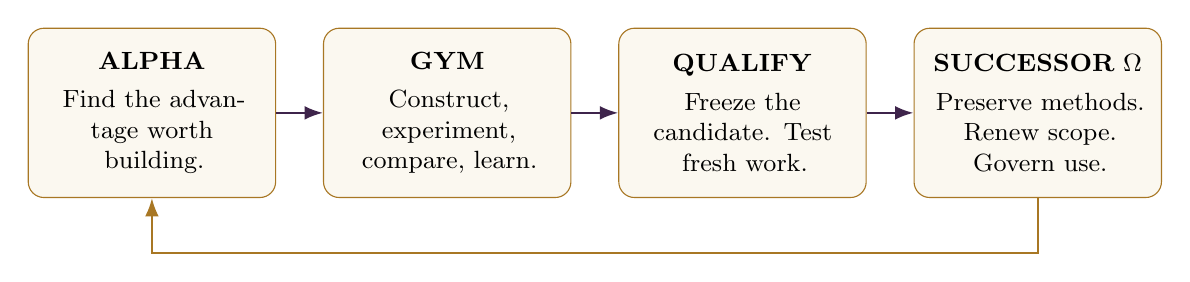
\begin{tikzpicture}[>=Latex,every node/.style={font=\small},
 card/.style={draw=Gold,fill=Ivory,rounded corners=2mm,text width=2.65cm,minimum height=2.15cm,align=center,inner sep=7pt}]
\node[card] (a) at (0,0) {\textbf{ALPHA}\\\smallskip Find the advantage worth building.};
\node[card] (b) at (3.75,0) {\textbf{GYM}\\\smallskip Construct, experiment, compare, learn.};
\node[card] (c) at (7.5,0) {\textbf{QUALIFY}\\\smallskip Freeze the candidate. Test fresh work.};
\node[card] (d) at (11.25,0) {\textbf{SUCCESSOR $\Omega$}\\\smallskip Preserve methods. Renew scope. Govern use.};
\draw[->,thick,Violet] (a)--(b);\draw[->,thick,Violet] (b)--(c);\draw[->,thick,Violet] (c)--(d);
\draw[->,Gold,thick] (d.south)--++(0,-.7)-|(a.south);
\end{tikzpicture}
\caption{Institutional continuity is the continuity of purpose, lawful assets, methods, and evidence---not automatic inheritance of approval across model changes.}
\end{figure}

The Gym develops capability; it does not certify itself. Qualification grants only the scope supported by the evidence. The term ``Specialist ASI'' in the conceptual visual material is not an achieved claim in this release. Superior performance on a named mission would require an appropriate comparison; it would not establish general superintelligence.

The institution retains qualified operations, representations, experiments, lessons, and operating history. It may replace a model without discarding everything legitimately learned. But model or environment changes can invalidate an analysis, integration, or acceptance bridge. Inheritance therefore carries applicability conditions, not permanent truth or unrestricted authority.

Generated code, external documents, and retrieved sources are untrusted inputs to execution. They must not modify the authority that controls secrets, payments, protected data, or promotion. The same principle applies to proposals for improving the controller: they can be constructed and evaluated, but cannot self-activate to approve the proposal that generated them. Authorized revision remains possible without circular certification.

\begin{keyidea}
Own the institution. Replace the models. Preserve the mission.\\
Retain what remains useful; requalify what has changed.
\end{keyidea}

\section{From discovery to expanding productive capacity}\label{sec:horizon}
The long horizon is larger than digital deliverables. Better observation can support better process models; those models can support more efficient or reliable production; production can create new instruments, energy systems, and infrastructure. Intellectual progress becomes materially consequential when it changes what can be built, maintained, and economically used.

The sequence is neither fixed nor guaranteed. Several intermediate constructions may be jointly necessary. A later invention may bypass a step assumed essential. A scientific instrument can be valuable through its contribution to downstream work without being independently profitable. The complete enabling chain still has to bear its costs and demonstrate its claimed relationships.

For a specified class of qualified productive units, write the stock relation as $\dot K=b-d$, where $b$ is commissioning rate and $d$ is retirement or loss. If each new unit requires energy $E_K$, material $M_K$, fabrication, and qualification, then a necessary dimensional bound is
\begin{equation}
b\leq\min\left\{\frac{P_{\mathrm{available}}}{E_K},
\frac{\dot M_{\mathrm{available}}}{M_K},b_{\mathrm{fabrication}},b_{\mathrm{qualification}}\right\}.
\label{eq:physical}
\end{equation}
All terms are expressed as units per time, with power and material flows actually available in the required forms. This is an accounting constraint under declared production assumptions, not a universal physical model. A new process can change the coefficients or the required inputs. It cannot turn predicted profit into absent materials, fabricate unqualified spare parts by assertion, or ignore heat rejection and maintenance.

The prospective progression extends from scientific instruments to materials and manufacturing, useful energy availability, robotic construction, and increasingly capable space-based productive systems. Its most ambitious horizon is stellar-scale productive reach: constructing the instruments and industrial capacity that make far greater use of available energy and matter possible. The paper supplies no deployment date, attained scale, or guaranteed wealth trajectory. These are separate construction programmes with physical uncertainty, ecological consequences, governance requirements, and competing uses of capital.

The enterprise objective should remain additional useful value through voluntary participation. Competitive diffusion may reduce private margins while increasing public benefit. Sustainable expansion should not depend on concealing risk, manufacturing customer dependence, or assuming that possession of intelligence confers entitlement to all value others create.

\section{Limitations and falsifiable commitments}\label{sec:limits}
The principal unresolved task is open-world discovery of economically meaningful possibilities. The current finite planner receives its markets, hypotheses, actions, costs, and observation laws. The composition engine receives its operation grammar. The native enterprise receives authored commercial assumptions and uses deterministic production. None establishes a live institution that sees the whole frontier or invents arbitrary new tools autonomously.

The framework also depends on measurement quality. Real scientific novelty can be difficult to judge; customer outcomes may be delayed; discovery value can be diffuse; and strong alternatives may change during a campaign. A low uncertainty estimate from an inadequate model is not adequate evidence. New hypotheses and changed representations can invalidate earlier calibration.

The three orders can fail independently. The observatory may miss a relevant development. The consequence generator may identify no valuable use or overestimate a chain of prerequisites. The planner may optimize the wrong economics. A retained method may be harder to maintain than to reconstruct. A successful application may offer no transfer. A new model may account for all apparent progress.



These conditions do not impose a ceiling on ambition. They make ambition operational. A small decisive experiment can address a large consequence; a large architecture without a decisive construction does not.

\section{Conclusion: the advantage that builds the next advantage}
ALPHA GENESIS FLYWHEEL $\Omega$ proposes an enterprise whose central skill is converting frontier progress into useful possibility. Its first order recognizes a real change in available means. Its second constructs the consequences that matter. Its third tests whether experience has improved the process that discovers those consequences.

The most important economic rule is origin neutrality. Use the strongest accessible existing means when they win. Construct only when the complete prospective value justifies the commitment. Retire unsupported or uneconomic inheritance. Preserve the distinction between commercial success, a useful invention, and a better inventor.

The executed evidence is intentionally narrower than the horizon. Exact finite planning selects experiments, existing agents, or non-entry as the conditions warrant. Native operation produces checked artifacts, records simulated collections, preserves obligations, and funds a research trial without inventing another ledger. The strong conventional method ties and remains in use. These are working foundations, not the completed discovery enterprise.

The decisive next achievement is a connected, independently tested lineage: a frontier change enables a valuable construction; the construction serves an accepted outcome; its retained means improve different fresh work; and the resulting economics support worthwhile continuation. Repeating that pattern would make the institution more than a beneficiary of stronger models. It would make it a productive participant in the creation of what comes next.

\begin{thesisbox}
\centering
{\large\bfseries See the frontier. See the consequences.\\Improve the machinery that sees possibilities.}\par\medskip
Invent the means. Expand what becomes possible.\\Compound the ability to discover.\par\medskip
{\large\bfseries\color{Violet}Build the advantage that discovers---\\and builds---the next advantage.}
\end{thesisbox}

\clearpage
\appendix
\section{Analytical details and interpretation}
\subsection{The finite diagnostic calculation}
In the base decision world, let $G$ denote successful construction. The probability of a positive signal is
\[
\Pr(+)=\frac{7}{20}\frac9{10}+\frac{13}{20}\frac1{10}=\frac{19}{50},
\qquad
\Pr(G\mid +)=\frac{63}{76},\quad \Pr(G\mid -)=\frac7{124}.
\]
After a positive signal, the remaining three steps allow construction and two deliveries. Conditional expected value from that state is $-12+(63/76)68+(13/76)30=49.5$. After a negative signal, using the frontier routes gives 30. The diagnostic's total value is therefore
\[
-3+\frac{19}{50}(49.5)+\frac{31}{50}(30)=34.41.
\]
Without the diagnostic, immediate construction yields $-12+(7/20)68+(13/20)30=31.30$, which the independent dynamic programme confirms is optimal among all allowed no-probe continuations. Simple direct delivery gives 30. With perfect initial information at no acquisition cost, the good world yields $68-12=56$, the bad world 30, and the weighted value is 39.10.

The signal's gross decision benefit relative to the no-probe planner is $6.11$ before paying its cost of 3; the net benefit is 3.11. Perfect information improves by 7.80. These inequalities are coherent with the information comparison: a noisy signal does not exceed free perfect knowledge under these assumptions. The signal also consumes time, already included in the four-step decision model.

The computation gives ordinary exact Bayesian planning the same actions and information. It therefore establishes a correct model-contingent decision, not superiority of a new planning algorithm. A misspecified prior, imperfect construction test, additional hidden market, changed horizon, or strategic rival response defines a different problem.

\subsection{Scope of the sensitivity comparison}
The 54 checks cross prior viability $\{1/10,7/20,4/5\}$, construction cost $\{4,12,16\}$, carrying cost $\{0,10,25\}$, and signal sensitivity $\{1/2,9/10\}$. The false-positive rate remains $1/10$; other base settings remain fixed. Both implementations permit only financially feasible experiments and construction. The tested agreement concerns optimal expected value; tie-breaking among equally valuable actions need not be a scientific distinction.

The oracle is separately coded but not an independent organization or a separately validated model of reality. It reduces the risk of a shared implementation mistake in the exercised transitions; it does not validate authored assumptions. All cases, including ones selecting no construction, remain in the output.

\subsection{Prospective retirement versus lifecycle attribution}
For remaining use count $R$, per-use saving $s$, integration $K$, and carrying cost $M$, the simple prospective comparison is $Rs-K-M$. An already incurred construction cost is sunk for this decision. For the separate claim that acquiring the asset was worthwhile, add the original construction and search costs back into the lifecycle account. The different comparisons answer different questions; neither authorizes hiding a failed investment.

A jointly useful bundle requires a comparison against the best alternative bundle, not a sum of independent asset scores. Likewise, one successor benefit must not be credited in full to each of several necessary ancestors and then summed as if it occurred several times. Lineage attribution can remain nonadditive while the cash account stays exact.

\subsection{Conditional adoption advantage}
Equation~\eqref{eq:lag} compares two institutions under a common assumed exponential capability path. It can be rewritten as $\log(Y_A/Y_B)=\log(\eta_A/\eta_B)+g(\tau_B-\tau_A)$. A lower conversion efficiency can outweigh a lag advantage. If a prerequisite bottleneck caps realized output, the ratio need not describe actual delivery. If a rival receives the same improvement, economic advantage additionally depends on value capture and outside options. No exponential revenue or intelligence law follows from this identity.

\section{Reproduction, source identity, and evidence}
\subsection{Run the self-contained analytical companion}
The paper package contains the finite decision model, the independently implemented oracle, unit tests, and retained exact results. Python's standard library is sufficient; no network, API key, model access, payment, or GPU is required.
\begin{lstlisting}
cd analysis
python3 -m unittest -v
python3 exact_studies.py --out ../my_exact_studies.json
\end{lstlisting}
The output path must be new. Compare its content with \sourcefile{evidence/exact_studies.json}. The independent oracle and the original planner are both available for inspection. The scenario inputs are in the code's explicit configuration; they are not inferred from current markets.

\subsection{Native reproduction requires its exact reference}
The native reproduction is separate from the paper's small analytical module. The source package includes the corrected Native Enterprise 002 additions, the historical public native source archive, and a reproduction driver. Its provenance record binds their hashes and the executing source identities. The native account's canonical funding and recovery machinery must not be replaced with a new balance simulation merely to obtain the reported result.

The bundled driver expands these sources into a new working directory, runs the native suite and the four account reproductions, and keeps local recovery authority out of the publication folder:
\begin{lstlisting}
python3 reproduction/reproduce_native.py --work /absolute/new/reproduction
\end{lstlisting}
It installs nothing. Its README states the pinned reference dependencies and POSIX requirement. From that exact reference plus the additive changes, the underlying commands are:
\begin{lstlisting}
python3 -m unittest discover -s tests \
  -p 'test_genesis002_*.py' -v
python3 -m genesis002 run \
  --config campaign/genesis-enterprise-002/INPUT.json \
  --output /absolute/new/genesis-run
python3 -m genesis002 audit --output /absolute/new/genesis-run
python3 -m genesis002 resume --output /absolute/new/genesis-run
\end{lstlisting}
The three stress cases are separately initialized accounts with the declared configuration and stress option. Do not combine their funds or interpret an account reproduction as a continuation of a historical operation. Operating directories contain local simulation authority and recovery state; they are not included in this publication package.

The safe evidence files report source-bound checks, not a transferable grant of account authority. The native results refer to commit \texttt{4a87b455373be72811ad3a0c654a116c3604a374}. The programme README was separately inspected at later commit \texttt{4f197eed10ddafc34f5a35968d93a1487815d0e1}. Reading the latter is not testing compatibility with it.

\subsection{Build and inspect the paper}
\begin{lstlisting}
pdflatex -interaction=nonstopmode -halt-on-error \
  ALPHA_GENESIS_FLYWHEEL_OMEGA_v2.tex
bibtex ALPHA_GENESIS_FLYWHEEL_OMEGA_v2
pdflatex -interaction=nonstopmode -halt-on-error \
  ALPHA_GENESIS_FLYWHEEL_OMEGA_v2.tex
pdflatex -interaction=nonstopmode -halt-on-error \
  ALPHA_GENESIS_FLYWHEEL_OMEGA_v2.tex
\end{lstlisting}
The supplied \texttt{build.py} automates the same build and handles the available BibTeX executable. The manuscript uses standard TeX Live packages and vector figures. The release includes a checksum manifest, build and layout checks, test transcripts, source provenance, and a claim register. File identity checks establish bytes, not scientific truth, correct consent, or data independence.

\section{Source lineage and responsible interpretation}
This edition develops the three-order framing and origin-neutral enterprise rule from the author's research discussions, the Transformational Intelligence manuscript, the prior GENESIS paper, and the supplied decision and native implementation packages. Those source discussions are intellectual provenance; their earlier narratives are not substitutes for inspected artifacts or new execution. The institutional figure adapts the Alpha--Gym--qualification--SUCCESSOR structure in the author-supplied visual material.

The new contribution is an integrated, falsifiable enterprise synthesis, a sharper discovery-versus-selection contract, the stronger finite information comparison, and source-matched verification of the supplied operational component. The elementary propositions use established decision and accounting reasoning. No claim is made to originate Bayesian planning, reinforcement learning, experimental design, program synthesis, or the broad idea of self-improvement.

External research results are credited to their authors. Availability statements are dated observations and may change. The paper does not claim external peer review, third-party certification, a tested world model of the economy, or any newly achieved general AGI/ASI threshold. AI assistance was used in research synthesis, drafting, implementation checking, and publication preparation; independent scientific and commercial claims still require their stated evidence.

The delivered paper and analytical companion do not modify a repository, operate customer equipment, contact buyers, activate billing, or initiate transactions. Publication readiness and enterprise qualification are distinct. A future claim of an operating GENESIS institution must release its own exact implementation, permitted interfaces, full campaign evidence, and accepted outcomes.


\clearpage
\section{Claim--evidence register}
\small
\begin{longtable}{P{.8cm}P{4.3cm}P{6.0cm}P{4.0cm}}
\caption{The strongest claim supported by each evidence class. Detailed machine-readable records accompany the release.}\label{tab:claims}\\
\toprule
\textbf{ID}&\textbf{Claim}&\textbf{Evidence}&\textbf{Boundary}\\
\midrule\endfirsthead
\toprule\textbf{ID}&\textbf{Claim}&\textbf{Evidence}&\textbf{Boundary}\\\midrule\endhead
C1 & Three-order enterprise architecture is specified. & Sections~\ref{sec:orders}--\ref{sec:institution}; explicit operating and evaluation contracts. & Proposal; not deployed general discovery.\\
C2 & The diagnostic is preferred in the base finite decision world. & Exact result 34.41; independent no-probe value 31.30; separately coded recursion. & Authored probabilities, actions, payoffs, and horizon.\\
C3 & Existing tools and non-entry can correctly win. & Frontier, carrying-cost, and no-market counterexamples; reproducible tests. & Does not estimate actual market-optimal choices.\\
C4 & Planner implementations agree over the disclosed sensitivity grid. & 54 cases; exact rational values; 15 analytical tests. & Agreement within the supplied family, not model calibration.\\
C5 & Native simulated operation is reproducible on its recorded reference. & Four six-cycle runs; local audit and unchanged resume; 62 native tests. & Historical source; no current-main or hosted release qualification.\\
C6 & The central native case records US\$143.20 modeled profit. & US\$240 receipts less US\$54.76 operating cost, US\$37.04 provision, US\$5 research. & Synthetic demand and cost envelopes; actual lifecycle costs unmeasured.\\
C7 & Some continuation uses native unrestricted simulated earnings. & Five repeat productions and one research purchase are funded EARNED. & Seed still backs protection reserves; not seed-independent operation.\\
C8 & The tested router does not demonstrate superiority over the strong conventional method. & Both accept 24 cases with identical mapping-work count 1,216; conventional method retained. & Mapping work is not total cost; no better-inventor claim.\\
C9 & Relevant external frontier advances are documented. & Dated primary sources and source/access distinctions in Table~\ref{tab:frontier}. & Provider reports and papers do not validate GENESIS.\\
C10 & Fast qualified conversion can matter under the exponential-lag model. & Equation~\eqref{eq:lag} and Appendix A. & Conditional algebra, not a fitted growth or profit forecast.\\
C11 & Open-world opportunity discovery, real commercial self-sustainability, and recurring inventor improvement are targets. & Registered tests and falsifiers specified; not yet satisfied by this release. & Explicitly unestablished.\\
\bottomrule
\end{longtable}
\normalsize

\clearpage
\small
\raggedright
\setlength{\bibsep}{6pt plus 1pt}
\interlinepenalty=10000
\bibliographystyle{plainnat}
\bibliography{references}
\end{document}
